Due to the presence of numerous physical, chemical, and physiological processes, vascular flow represents a highly complex process. In many cases, however, a simplified model that neglects some characteristics suffices for its description \cite{Saloner2019}. In this section, we briefly describe some aspects for which a simplified model can be considered under appropriate assumptions.

\section*{\fontsize{11}{15}\selectfont Elasticity of Walls}
The interaction of an elastic body, i.e., a body with a movable boundary, can be modeled, for example, using the immersed boundary method \cite{Peskin}. In many cases, however, the elasticity of wall obstacles can be neglected, and only rigid geometry considered. Particularly in smaller vessels, neglecting the elasticity of the vascular walls has not shown a significant effect on the outcome. \cite{DempereMarco2006} However, this is not always the case, as significant non-negligible effects on the overall error of the results have been observed in the area of the aorta when considering rigid geometry. \cite{LANTZ2011}

Note that including the elasticity of vascular walls in the considered model requires appropriately defining the conditions of interaction with the fluid, which is generally a difficult task in vascular flow, often depending on the correct evaluation of \textit{in vivo} measurements. Additionally, in diseases such as arteriosclerosis\footnote{Arteriosclerosis is a disease in which the arterial walls thicken and subsequently lose their elasticity \cite{Fishbein2015}.}, vessels lose their elasticity in many patients, thus including elasticity in the model may not necessarily reflect the physiological state of the vessels correctly \cite{Saloner2019}.

\section*{\fontsize{11}{15}\selectfont Blood Viscosity}

For the mathematical model, it is important to choose the viscosity values correctly to encompass any non-Newtonian behavior of the fluid under investigation. Blood is generally considered a Newtonian fluid. However, there are situations where the Newtonian behavior of blood is compromised. For instance, in cases where the flow velocity of blood is very low, red blood cells can accumulate, consequently increasing the viscosity of blood.
Areas with such slow flow can be found, for example, in regions of aneurysmatic dilation\footnote{Aneurysmatic dilation refers to a disease condition where there is a local enlargement of a vessel \cite{Syed1997}.}. On the other hand, the viscosity of blood significantly decreases in areas where blood flows through very narrow vessels, particularly through vessels at the scale of arterioles or capillaries \cite{Saloner2019}.

There are viscosity models that aim to more accurately capture the physical description and behavior of blood viscosity~\cite{Saloner2019, Eichler2023, Boyd2007}. The simplest is the so-called Power-Law model \cite{Sequeira}. The Power-Law model prescribes for viscosity
\begin{equation}\label{eq:power-law}
	\mu _{\text{PL}} (\dot{\gamma}) = K_p  \dot{\gamma} ^{n_1-1} \ ,
\end{equation}
where $ K_p$ \si{[kg.m^{-1}]} and $ n_1 $ \si{[-]} are constants. Another model is the Casson model \cite{Boyd2007} which satisfies
\begin{equation}\label{eq:Casson}
	\mu _{\text{CA}} (\dot{\gamma}) = \frac{1}{\dot{\gamma}} \left[ k_{0} + k_{1} \sqrt{\dot{\gamma}} \right]^2 \ ,
\end{equation}
where $ k_1$ \si{[kg^{2}.m^{-2}]} and $ k_2 $ \si{[kg^{2}.m^{-2}]} are empirically determined constant parameters. A major advantage of these basic models is that for certain geometries and under specific conditions, exact solutions are available, which for example, provide reference values for numerical simulations. An obvious disadvantage of these models is their limited applicability, as they fail for shear rates approaching zero \cite{Boyd2007}.

Among the more complex models, the Cross model \cite{Sequeira} is defined by the relation
\begin{equation}\label{eq:cross}
	\mu _{\text{CR}} (\dot{\gamma}) = \frac{\mu_{0} - \mu_{\infty}}{1 + (k\dot{\gamma})^{n_2}} + \mu_{\infty}  \ ,
\end{equation}
where $ k $ \si{[s]} and $ n_2 $ \si{[-]} are constants, and it is also valid that
\begin{equation}\label{eq:m0 a minf}
	\mu _{0}  = \lim_{\dot{\gamma} \rightarrow 0+}\mu (\dot{\gamma})\, , \ \mu_{\infty} = \lim_{\dot{\gamma} \rightarrow \infty}\mu (\dot{\gamma}).
\end{equation}
The last mentioned model is the Carreau-Yasuda model \cite{Boyd2007} satisfying
\begin{equation}\label{eq:C-Y}
	\mu _{\text{CY}} (\dot{\gamma}) = \mu_{\infty} + (\mu_{0} - \mu_{\infty}) \left[ 1 + (\varepsilon \dot{\gamma}) ^{a} \right]^{\frac{n_3-1}{a}} \ ,
\end{equation}
where $ \varepsilon$ \si{[s]} , $a$ \si{[-]}, and $ n_3 $ \si{[-]} are again empirically determined constant parameters that influence the model behavior between boundary viscosity values. For $ \mu_{0}$ and $ \mu_{\infty} $ the condition \eqref{eq:m0 a minf} still applies.

All mentioned models are compared in Fig. \ref{fig:vs}, with parameter values taken from \cite{Eichler2023}.
\begin{figure}[H]
	\centering
	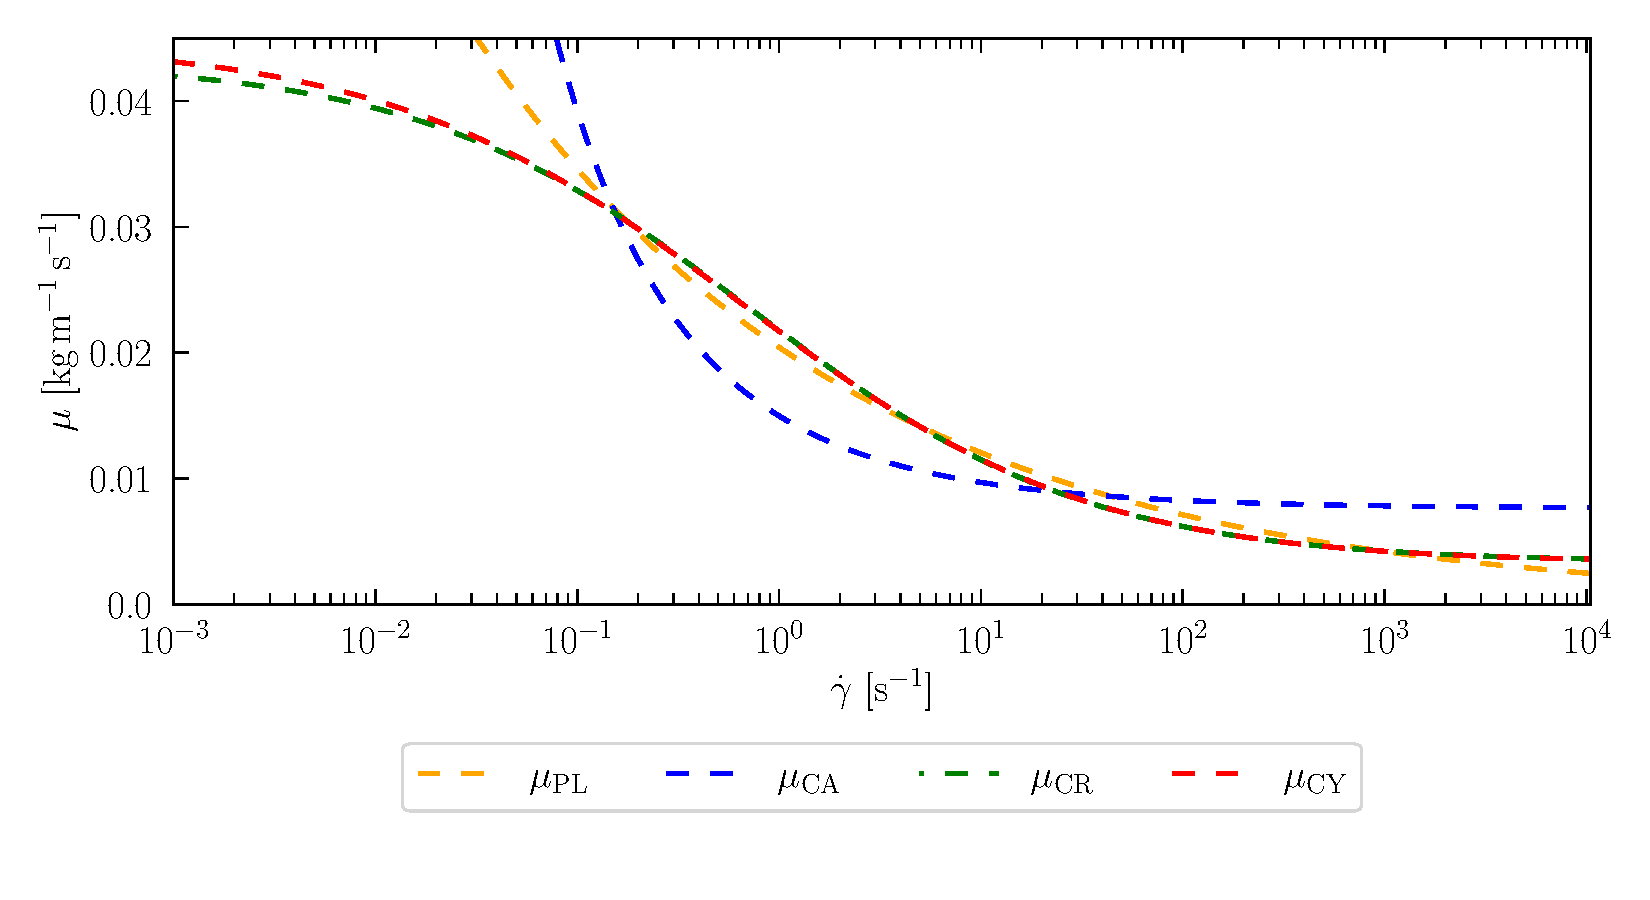
\includegraphics[width=1.0\textwidth]{figures/modely.pdf}
	\vspace{-9mm}
	\caption{Comparison of non-Newtonian viscosity models, specific parameter values were taken from \cite{Eichler2023}. Descriptions of each model correspond to the defining equations
		\eqref{eq:power-law}, \eqref{eq:Casson}, \eqref{eq:cross}, and \eqref{eq:C-Y}.}
	\label{fig:vs}
\end{figure}
We note that in this work, blood will be considered exclusively as a Newtonian fluid.

\section*{\fontsize{11}{15}\selectfont Turbulent Flow}
In most cases, blood flow can be approximated by laminar flow \cite{Sequeira}. However, in some instances in vascular flow, turbulence and chaotic behavior occur \cite{Saqr2020}. One area where turbulence can be observed is behind a vascular stenosis\footnote{Vascular stenosis is a condition in which there is a local narrowing of a vessel \cite{Carabello2009}.} \cite{Jain2022}. The flow velocity of blood in the narrowed area can significantly increase, and the reduction in the diameter of the vessel ensures that the flow remains laminar in this section of the constriction \cite{Sequeira}. However, immediately after the constriction, the flow velocity remains elevated even in areas with the original diameter, which can lead to the formation of vortices and a change in flow regime \cite{Saloner2019, Varghese2003}.

The occurrence of turbulent flow is physiologically undesirable as it is often accompanied by significant dissipation of kinetic energy, which can strain parts of the circulatory system. Additionally, vascular areas with turbulence show increased strain on vessel walls, which can lead to tissue damage and diseases such as arteriosclerosis. Therefore, it is desirable to minimize turbulence in blood flow \cite{Saloner2019, Kameneva2004}.